\usetikzlibrary{shapes.geometric, arrows}

\tikzstyle{startstop} = [rectangle, rounded corners, 
minimum width=3cm, 
minimum height=1cm,
text centered, 
draw=black, 
fill=red!30]

\tikzstyle{io} = [trapezium, 
trapezium stretches=true, % A later addition
trapezium left angle=70, 
trapezium right angle=110, 
minimum width=3cm, 
minimum height=1cm, text centered, 
draw=black, fill=blue!30]

\tikzstyle{process} = [rectangle, 
minimum width=3cm, 
minimum height=1cm, 
text centered, 
text width=3cm, 
draw=black, 
fill=orange!30]

\tikzstyle{decision} = [diamond, 
minimum width=3cm, 
minimum height=1cm, 
text centered, 
draw=black, 
fill=green!30]
\tikzstyle{arrow} = [thick,->,>=stealth]

%%
% \newacronym{cad}{CAD}{computer-aided design}
% \newacronym{pid}{PID}{proportional–integral–derivative}
% \newacronym{dnn}{DNN}{Deep Neural Network}
% \newacronym{lqr}{LQR}{linear-quadratic regulator}
% \newacronym{mpc}{MPC}{model predictive control}
% \newacronym{pd}{PD}{proportional–derivative}
%%

\fancyhead[C]{Samuel Grace}

\subsection{Overview}

In this section of the project, software was developed to simulate the multi-agent aerial robotic system. For a drone to be able to capture useful images, it is essential that the drone can hover with minimal disturbance to its position. Achieving this stability requires a controller to be designed that is robust to sensor noise and environmental disturbances. The development of the flight control system focused on ensuring that the \gls{uav} was sufficiently stable during a period of hovering, while also making the controller robust for general flight.

A \gls{bms} was designed to optimise the drone's performance, further extending the mission duration as well as providing other advantages discussed in Subsection \ref{}. The combination of the bespoke controller designed for the drone with the customised \gls{bms} components and algorithms provides an \gls{uav} that is ideally suited to detecting landmines in a wide variety of environmental scenarios.

The results obtained in this section were solely generated from simulations run within the C, Python, MATLAB, Simulink and Simscape environments. These simulations provided insights into the operation of the drone using a cascade \gls{pid} controller designed specifically for the chosen drone.  Real-time environmental conditions were also modelled in the simulations. The controller would then be implemented onboard the drone using embedded C. The details of the hardware and software used to perform these simulations are outlined in Table \ref{tab:computersetup}. The ARM GNU Toolchain is used to test the C code developed for use onboard the drone.  
\begin{table}[h]
\begin{center}
\begin{tabular}{| p{6cm}|p{10cm}|}
 \hline
 \textbf{Specification}       & Details\\ 
 \hline
 Computer Model                & HP ENVY Laptop - 17-cg0002na          \\ 
 CPU Type                     & Intel Core i7-1065G7 with 4 cores, up to 3.90 GHz \\ 
 Operating System and Version & Windows 11 Home, Version 23H2, OS Build 22631.4460 \\ 
 Memory (RAM)                 & 16 GB DDR4-3200 SDRAM (2x8GB)      \\  
 Storage                      & HP 512GB PCIe NVMe M.2 SSD            \\ 
 MATLAB Version               & 24.2.0.2712019 (R2024b) \\ 
  Python Version& Python 3.12.1\\
 C Version&C17 (ISO/IEC 9899:2018)\\ 
 GNU Toolchain& ARM GNU Toolchain 12.3.Rel1 (for STM32H7)\\ 
 \hline
\end{tabular}
\end{center}
\caption{Computer hardware and software specifications.}
\label{tab:computersetup}
\end{table}

Figure \ref{fig:simctrloverview} shows the overall scheme of the Simulation and Control process. First, the location coordinates were passed into the software, to enable environmental, weather and climate effects to be accurately modelled. Next, the \gls{cad} model of the drone was analysed to accurately represent the drone's dynamics within the simulation.

An iterative simulation and optimisation process was then used to determine the controller parameters for the cascade \gls{pid} controller used. These steps made use of the Meteomatics API to provide accurate weather data, as discussed in Section \ref{ab}. Deployment of the optimised controller was then simulated in conjunction with the \gls{bms} to ensure that the drone has adequate battery capacity for the planned mission. 

Once a single drone had been modelled, the simulation was then extended to model the multi-agent operation in the presence of motor nonidealities and environmental disturbances. The increased complexity introduced by this approach was worthwhile since it provided additional confidence that each agent could carry out their mission while maintaining a safe distance from other agents. The controller parameters could then be uploaded to the drone instantaneously; the structure of the cascaded \acrshort{pid} controller is fixed so the loop gains could simply be uploaded to the microcontroller as floating-point numbers.



\begin{figure}[H]
\centering
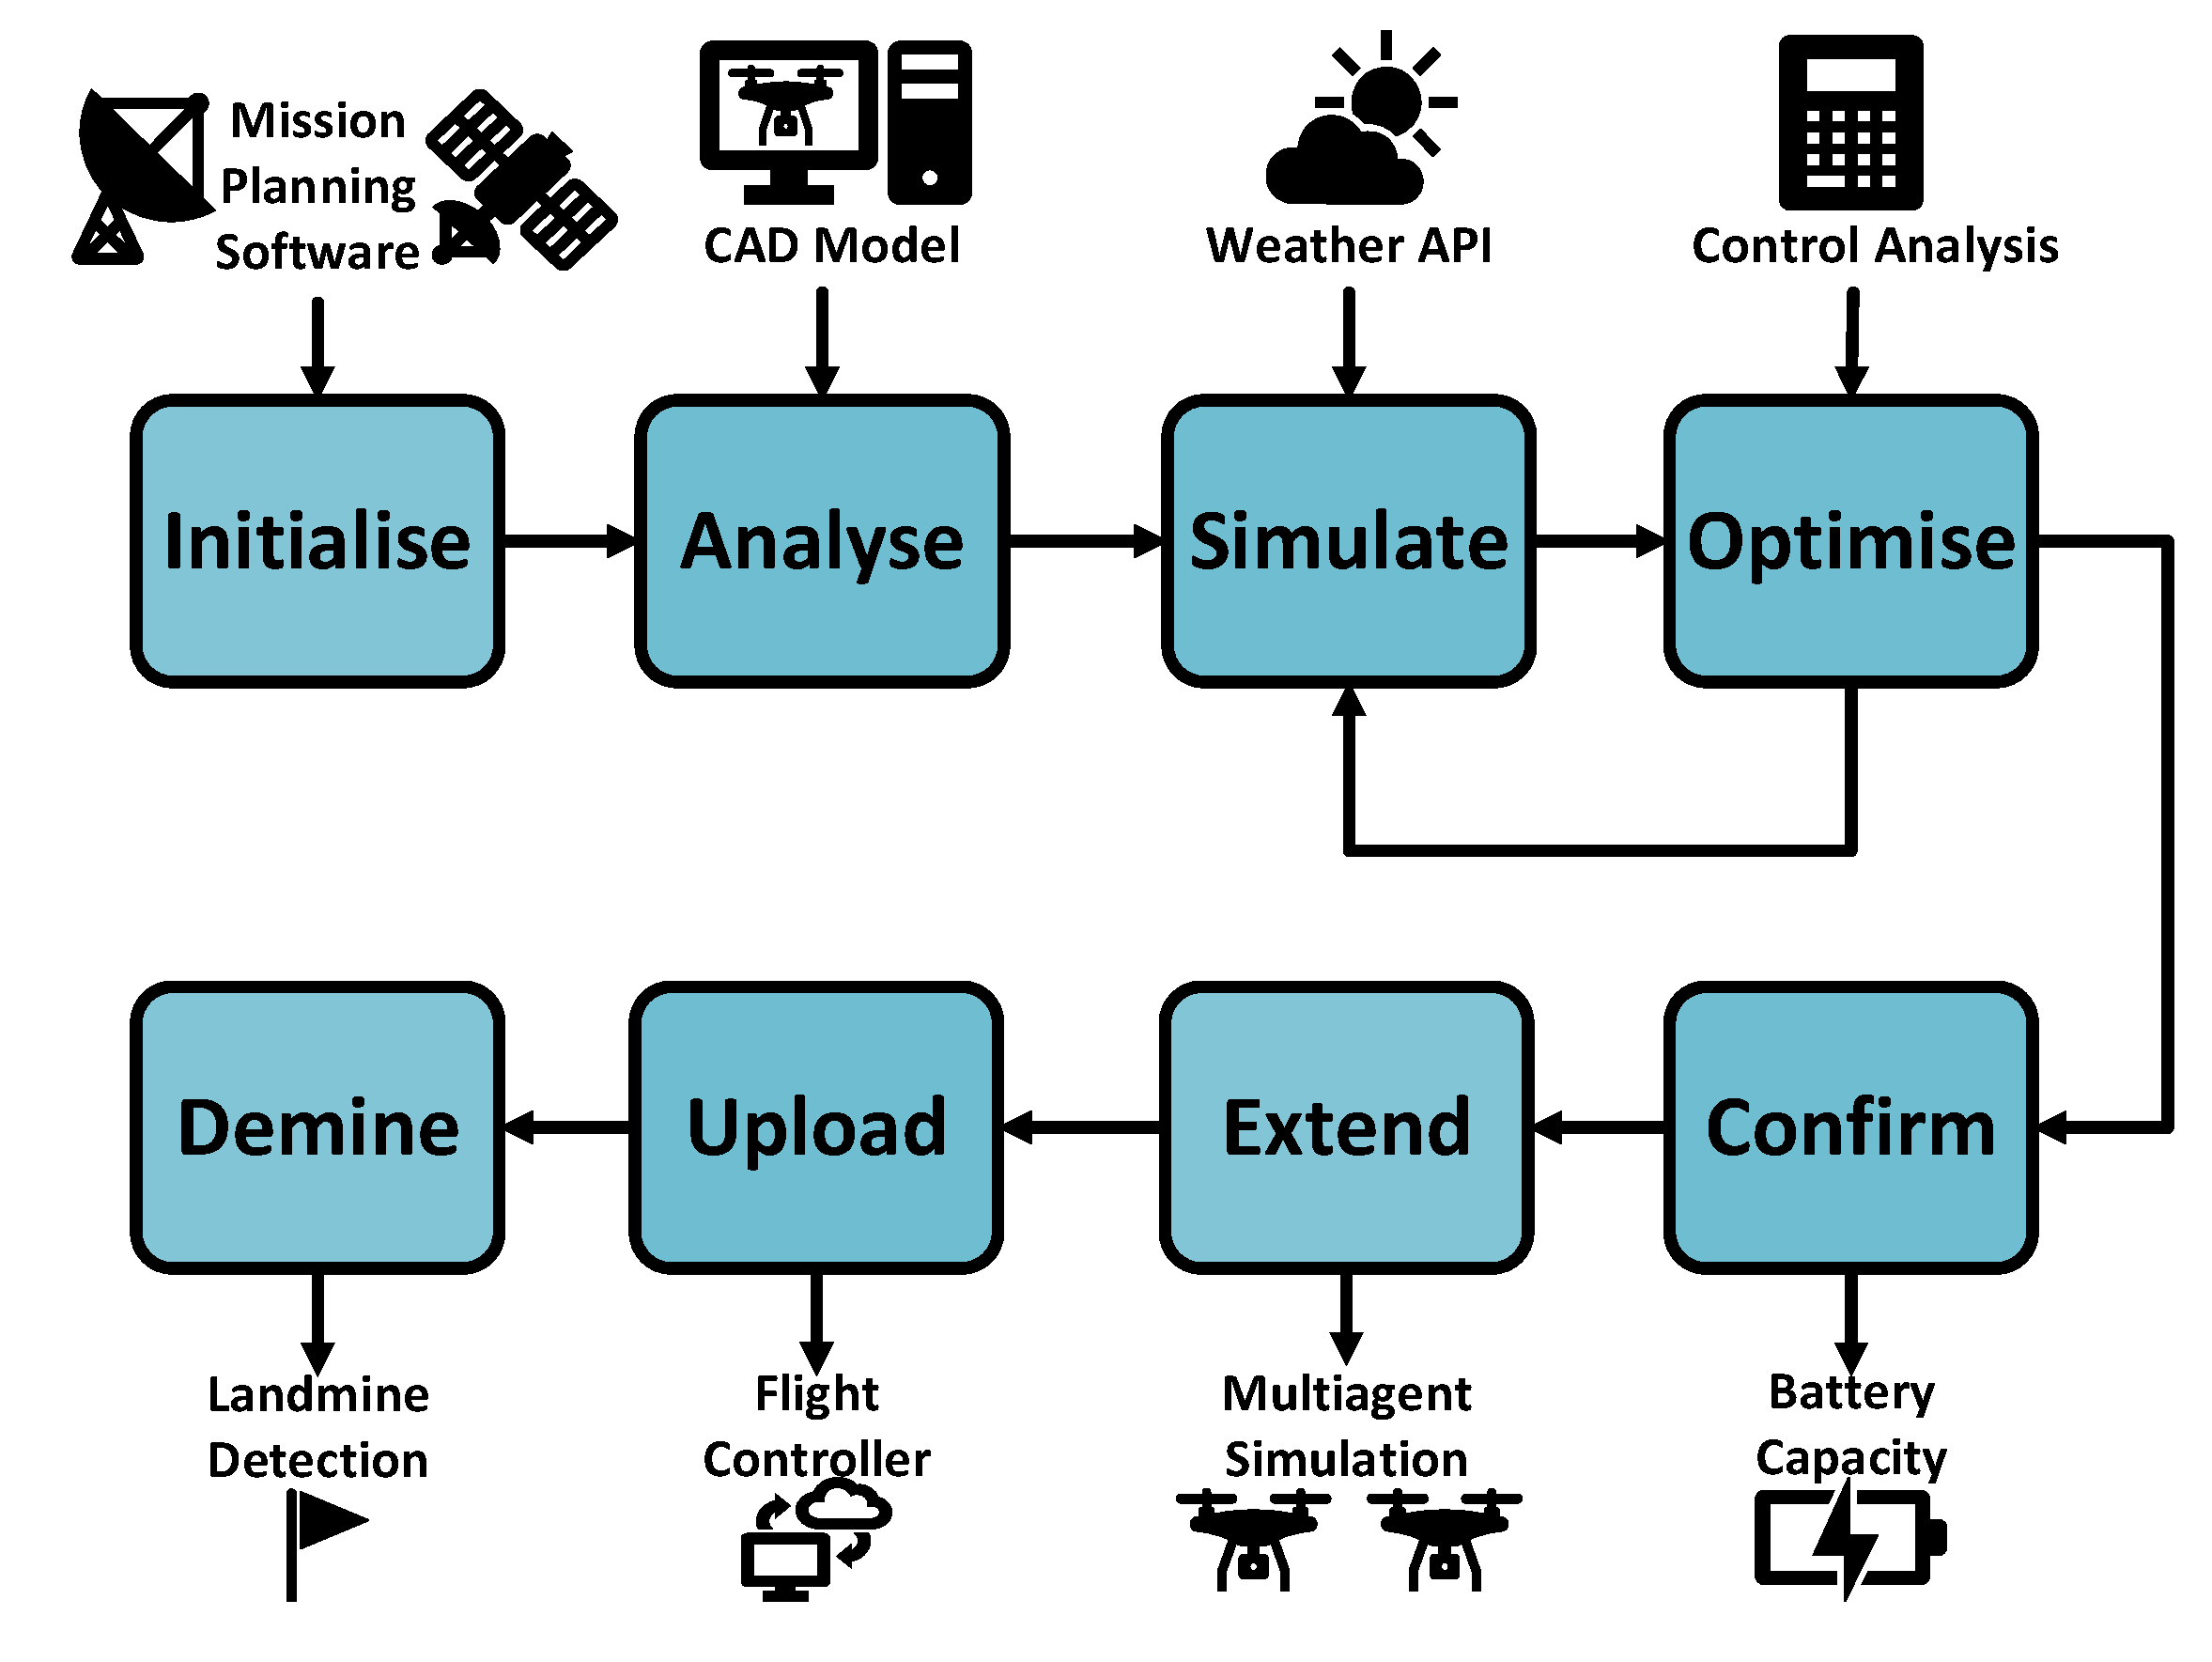
\includegraphics[width=0.86\textwidth]{figs/Samuel/Figures/Sim and Control Overview BASIC1.pdf}
\caption{Simulation and Control Overview}
\label{fig:simctrloverview}
\end{figure}





\subsection{Physical Modelling of the Drone Using CAD}
\label{cad}

To simulate the drone's dynamics, it is important to have an accurate model of the drone's physical properties. These include its mass, inertia tensor and the position of its centre of gravity. The drone has sensors attached and the effects of these sensors on the drone's dynamics need to be modelled. This necessitated the development of a \textbf{Computer Aided Design (CAD)} model for the quadcopter. The model was rendered in SolidWorks, and an existing model \cite{westin2019x4} is used as the basis for the quadcopter design. Figure \ref{fig:dronecad} shows the model of the drone. 

A key benefit of this approach is the ability to automatically generate the \textbf{mass properties} in SolidWorks, which includes all the necessary information for an accurate simulation of the drone. To create a drone with stable dynamics, it was essential to have symmetrically mounted components as shown in Figure \ref{fig:2a}. The sensors and onboard processors are also centrally located to ensure the drone is stabilisable when in the hovering position. The CAD model is also easily adaptable, should there be any modifications to the drone's sensors during its operational lifetime. The drone's \textbf{inertia matrix} is shown in Figure \ref{fig:2b}, which was generated automatically.

\begin{figure}[H]
    \centering
    \begin{subfigure}[b]{0.5\textwidth} % Left-hand side: Drone image
        \centering
        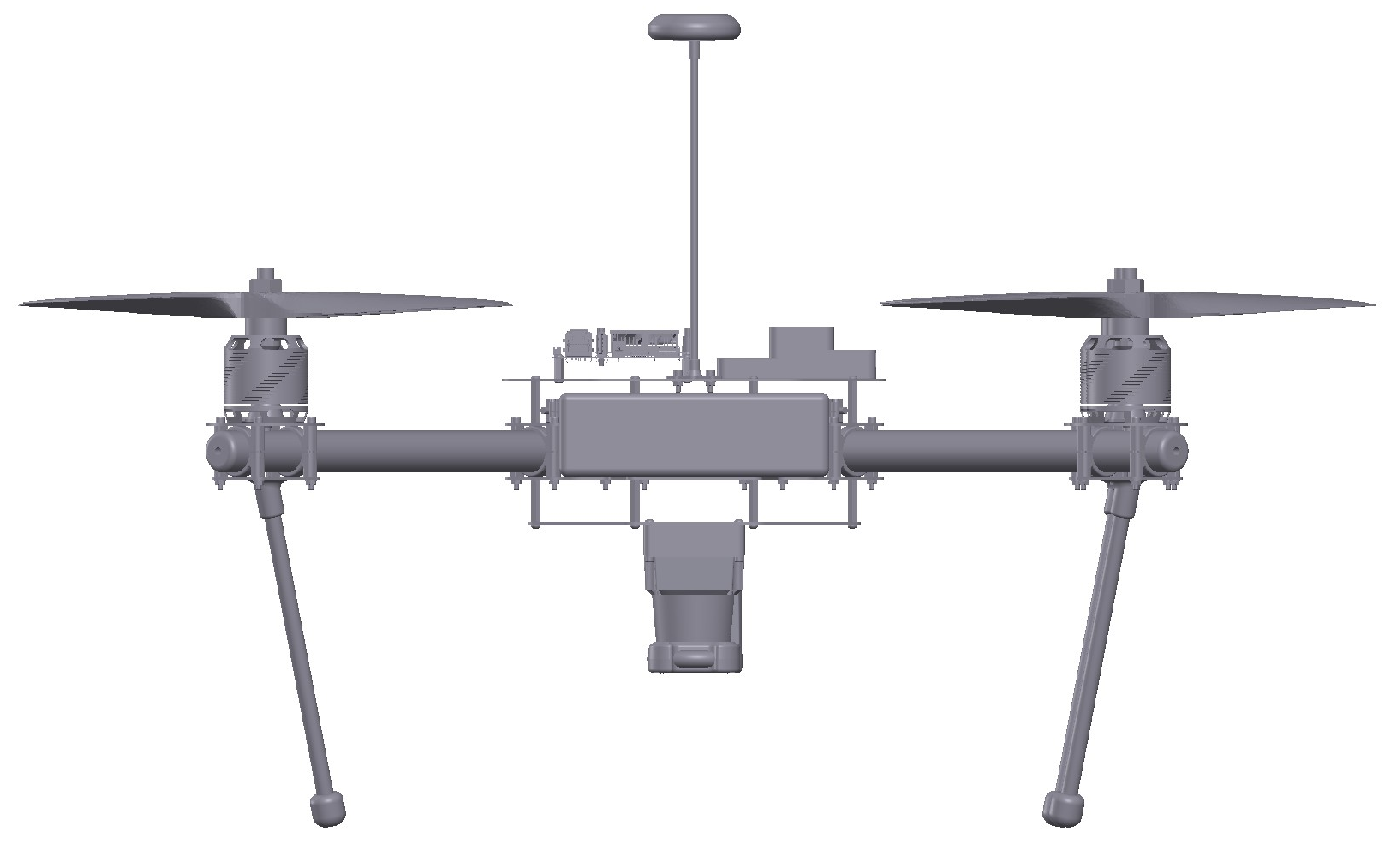
\includegraphics[width=\textwidth]{figs/Samuel/Figures/drone_new2 (cropped) (pdfresizer.com).pdf}
        \caption{}
        \label{fig:2a}
    \end{subfigure}
    \hspace{0.01\textwidth}
    \begin{subfigure}[b]{0.3\textwidth} % Right-hand side: Inertia matrix
        \centering
        \begin{equation*}
            \mathbf{I} =
            \begin{bmatrix}
                0.0875& 0.0002 & 0.0000 \\
                0.0002 & 0.0768 & 0.0185 \\
               0.0000 & 0.0185 & 0.0124
            \end{bmatrix} \quad \text{kg} \cdot \text{m}^2
        \end{equation*}
        \caption{}
        \label{fig:2b}
    \end{subfigure}
    \caption{CAD model of the UAV quadcopter in SolidWorks from \cite{westin2019x4} shown in (a), with the corresponding inertia matrix shown in (b).}
    \label{fig:dronecad}
\end{figure}


\subsection{Exploration of Control Strategies}

By using the mass properties modelled in Section \ref{cad}, it was possible to construct an accurate representation of the drone's dynamics, referred to here as the \textbf{Quadrotor Plant}. Figure \ref{fig:nekoodiag} shows the coordinate system used to model the drone, with both the \textbf{inertial frame} and \textbf{body frame} being used in the simulation. For the cascade \gls{pid} and \gls{lqr} designs, the altitude and linear velocities are taken from the inertial frame, whereas the attitude and angular velocities are taken from the body frame. The control inputs are the voltages supplied to the four rotors shown in Figure \ref{fig:nekoodiag}.


\begin{figure}[H]
\centering
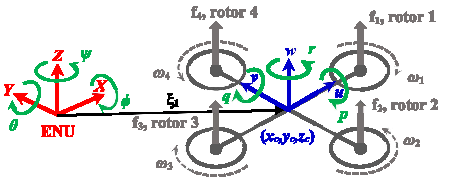
\includegraphics[width=0.71\textwidth]{figs/Samuel/Figures/nekoodiagram-cropped.pdf}
\caption{Diagram of the drone's dynamics in the inertial and body frames of reference. Diagram from \cite{nekoo}}
\label{fig:nekoodiag}
\end{figure}

\subsubsection{Cascade \gls{pid} Control}
Since cascade \gls{pid} is ubiquitous in commercial drones, the technique was considered first. The method involves constructing nested feedback loops, with the \textbf{Attitude Controller} located inside the \textbf{Position Controller} loop. A simplified representation of the cascade \gls{pid} scheme used in the drone is shown in Figure \ref{fig:pidloop}, as in reality the loops each have 3-dimensional states as inputs and outputs. A detailed description of the control strategy is given in an industrial review of cascade \gls{pid} control \cite{electronics10040376}.

\begin{figure}[H]
\centering
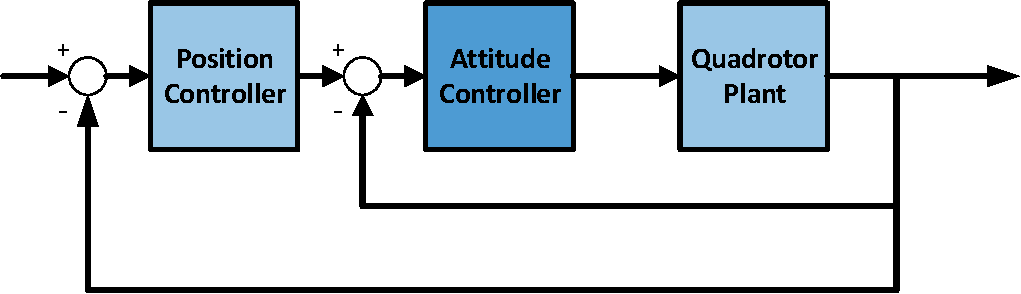
\includegraphics[width=0.75\textwidth]{figs/Samuel/Figures/Control Loop-cropped.pdf}
\caption{Cascade \gls{pid} control diagram (simplified)}
\label{fig:pidloop}
\end{figure}




\subsubsection{LQR with Integral Action}

In the hovering condition, position (\(x_c, y_c, z_c\)) and orientation (\(\phi, \theta, \psi\)) remain constant, with linear and angular velocities taken to be $\approx$ 0. By following the procedure outlined in \cite{cengiz2024quadcopter}, the linearised dynamics are obtained. This allows a Linear Quadratic Regulator (LQR) to be constructed for the system. An LQR is an optimal state-feedback controller, computed by minimising the cost function shown in Equation \ref{eq:cost_function}:

\begin{equation} \label{eq:cost_function}
J = \int_0^\infty \left( x^\top Q x + u^\top R u \right) \, dt 
\end{equation}

$Q$ and $R$ represent the running state and input penalties respectively. It is necessary to achieve a balance between minimising disturbances and having input demands that can reasonably be met by the actuators and battery, meaning that there is an inherent compromise between control effort and performance. As there is no set method for selecting the state and input costs, \textbf{Bryson's rule} is used to heuristically select appropriate diagonal $Q$ and $R$ matrices by setting $Q_{ii} = \frac{1}{\text{maximum acceptable}( [x_i]^2 )}$ and $R_{ii} = \frac{1}{\text{maximum acceptable}( [u_i]^2 )}$ where $[x_i]$ and $[u_i]$ are the states and inputs respectively \cite{chibum2014adv09designofsfb1}. These values are selected according to the drone's sensing capabilities and flight hardware. $Q$ and $R$ are then tuned iteratively to produce the final LQR controller design.

\subsubsection{Evaluation of Control Strategies}

Both strategies were implemented in Simulink, with the methods performing similarly in terms of overshoot and disturbance rejection. The \gls{lqr} had a slightly higher energy efficiency than the cascade \gls{pid} design, though this efficiency could be altered by adjusting the $Q$ and $R$ matrices in the \gls{lqr} design. Due to both controllers performing similarly well, computational complexity is the deciding factor. Both implementation and tuning of a \gls{pid} controller are simpler than for an \gls{lqr} controller, so cascade \gls{pid} was selected as the control scheme.

\subsubsection{Cascade \gls{pid} Analysis}

The strategy selected for implementation onboard the drone is cascade \gls{pid} control; this strategy is easily implemented using lightweight code on the microcontroller and can be readily optimised for any given weather and mass properties. Also, cascade \gls{pid} control is near ubiquitous within the \gls{uav} industry, which further suggests that it is a sensible choice. The model used for the MATLAB and Simulink simulations was modified from a cascade \gls{pd} implementation by Nekoo et al. \cite{nekoo}, by incorporating an integral term into each feedback loop.

The results produced are shown in Figure \ref{fig:nekpid}. Shortly after 2 seconds there are relatively large disturbances to the roll and pitch, which suggests a sudden gust of wind. The disturbance of up to 0.4 rad would be significant enough to invalidate sensor measurements, which suggests that more sophisticated disturbance rejection is required. This is discussed further in Section \ref{gust}. 



% \begin{figure}[H]
%     \centering
%     \foreach \i in {12,11,10,9,8,7,6,5,4,3,2,1} {
%         \begin{subfigure}[b]{0.28\textwidth} % Adjust width to fit 3 per row
%             \centering
%             \includegraphics[width=\textwidth, angle=180, page=\i]{Figures/Subplots/gvhbjnkml.pdf}
%             \captionsetup{justification=centering, margin={15pt,0pt}} % Adjust caption placement
%             \caption{}
%             \label{fig:subplot\i}
%         \end{subfigure}
%         \hspace{15pt} % Add horizontal space between subplots
%         \ifnum\i=10 \hspace{0pt} \vspace{10pt} \linebreak \fi
%         \ifnum\i=7 \hspace{0pt} \vspace{10pt} \linebreak \fi
%         \ifnum\i=4 \hspace{0pt} \vspace{10pt} \linebreak \fi
%     }
%     \caption{Effects of temperature variation on cell properties}
%     \label{fig:tempythings}
% \end{figure}

\textbf{INCLUDE GRAPH}





\newpage




\subsection{Control Tuning Process}

To provide a bespoke controller design for each mission, the method described by the flowchart in Figure \ref{fig:drone_flow_updated} was used to iteratively update the cascade \gls{pid} loop gains until a satisfactory controller had been successfully designed. The feedback loop ensured that the mission operator was aware of the performance capabilities of the drone; the mission duration can be varied if the environmental conditions necessitate a controller with a higher average power consumption. The \href{https://www.meteomatics.com/}{\textbf{Meteomatics API}} provides the necessary weather data for the given location, and Section \ref{cad} shows the model used to generate the drone's mass properties. The performance evaluation step involves both the system automatically confirming that no constraints were broken, and the operator manually reviewing graphs of the evolution of the drone's states. The two layers of verification provide additional confidence that the controller has been designed successfully. Finally, the selected loop gains are uploaded directly to the onboard microcontroller, so that the cascade \gls{pid} controller can be deployed on the \gls{uav}. 

\begin{figure}[H]
\centering
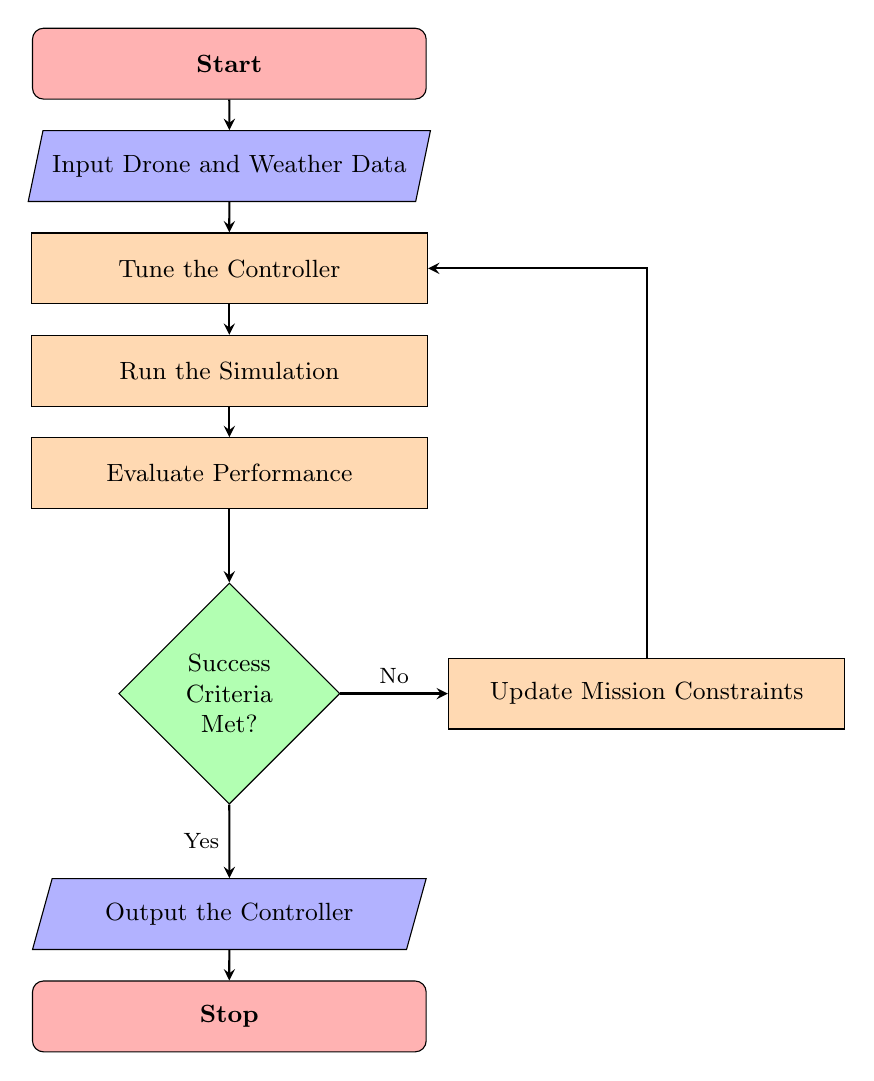
\begin{tikzpicture}[node distance=1.3cm, every node/.style={font=\small}]
% Define styles
\tikzstyle{startstop} = [rectangle, rounded corners,
minimum width=5cm,
minimum height=0.9cm,
text centered,
draw=black,
fill=red!30]

\tikzstyle{io} = [trapezium,
trapezium stretches=true,
trapezium left angle=70,
trapezium right angle=110,
minimum width=5cm,
minimum height=0.9cm,
text centered,
draw=black,
fill=blue!30]

\tikzstyle{process} = [rectangle,
minimum width=5cm,
minimum height=0.9cm,
text centered,
text width=4.8cm,
draw=black,
fill=orange!30]

\tikzstyle{decision} = [diamond,
minimum width=1.2cm,
minimum height=1.2cm,
text centered,
text width=1.35cm,
draw=black,
fill=green!30]

\tikzstyle{arrow} = [thick,->,>=stealth]

% Nodes
\node (start) [startstop] {\textbf{Start}};

\node (input) [io, below of=start, yshift=+0cm, align=center] {Input Drone and Weather Data};

\node (simulate) [process, below of=input] {Tune the Controller};

% Added "Optimize Controller" node
\node (optimize) [process, below of=simulate] {Run the Simulation};

\node (evaluate) [process, below of=optimize] {Evaluate Performance};

\node (decide) [decision, below of=evaluate, yshift=-1.5cm] {Success Criteria Met?};

\node (adjust) [process, right of=decide, xshift=4cm] {Update Mission Constraints};

\node (output) [io, below of=decide, yshift=-1.5cm, align=center] {Output the Controller};

\node (stop) [startstop, below of=output, yshift=+0cm] {\textbf{Stop}};

% Connections
\draw [arrow] (start) -- (input);
\draw [arrow] (input) -- (simulate);
\draw [arrow] (simulate) -- (optimize);
\draw [arrow] (optimize) -- (evaluate);
\draw [arrow] (evaluate) -- (decide);

\draw [arrow] (decide) -- node[anchor=east, xshift=-0cm] {\footnotesize Yes} (output);

\draw [arrow] (decide) -- node[anchor=south] {\footnotesize No} (adjust);

\draw [arrow] (adjust) |- (simulate);

\draw [arrow] (output) -- (stop);

\end{tikzpicture}
\caption{Flowchart of the iterative tuning process.}
\label{fig:drone_flow_updated}
\end{figure}






\newpage

\subsection{Mission Case Study for Kharkiv, Ukraine DATES LOCATION CHANGEM}

\textbf{INCLUDE DATA}
\subsection{Multi-Agent Simulations}

A key aspect of designing a \textbf{multi-agent} system is modelling the interaction between different agents, in this case quadcopters. The most crucial factor is collision avoidance, since any collision between drones would likely result in significant damage or destruction of the \gls{uav}s. For this reason, the simulation software was designed in MATLAB and Simulink to model the drones traversing the paths generated by the mission planning software, identifying if the drones are in too close proximity in the simulation. The software logs time instances when the drones are too close together, and also provides an animation of the drones carrying out the mission, as shown in Figure \ref{fig:dronemulti}. The animation displays the drones in green when they are operating at a safe separation distance, and in red when they are within an unsafe distance of another drone. 

The software can model an arbitrary number of drones operating simultaneously, and the threshold for the drones being a safe distance apart can be changed depending on the mission environment. The threshold distance used for the simulation in Figure \ref{fig:dronemulti} is 5 metres, and is a standard threshold used in multi-agent aerial robotics \cite{crannverdon}. This simulation models a theoretically safe mission computed in the mission planning software, and shows that even in near-ideal conditions, the drones end the mission within an unsafe distance of each other. 
 
\begin{figure}[H]
    \centering
    \begin{subfigure}[b]{0.48\textwidth} % Use [b] to align captions at the bottom
        \centering
        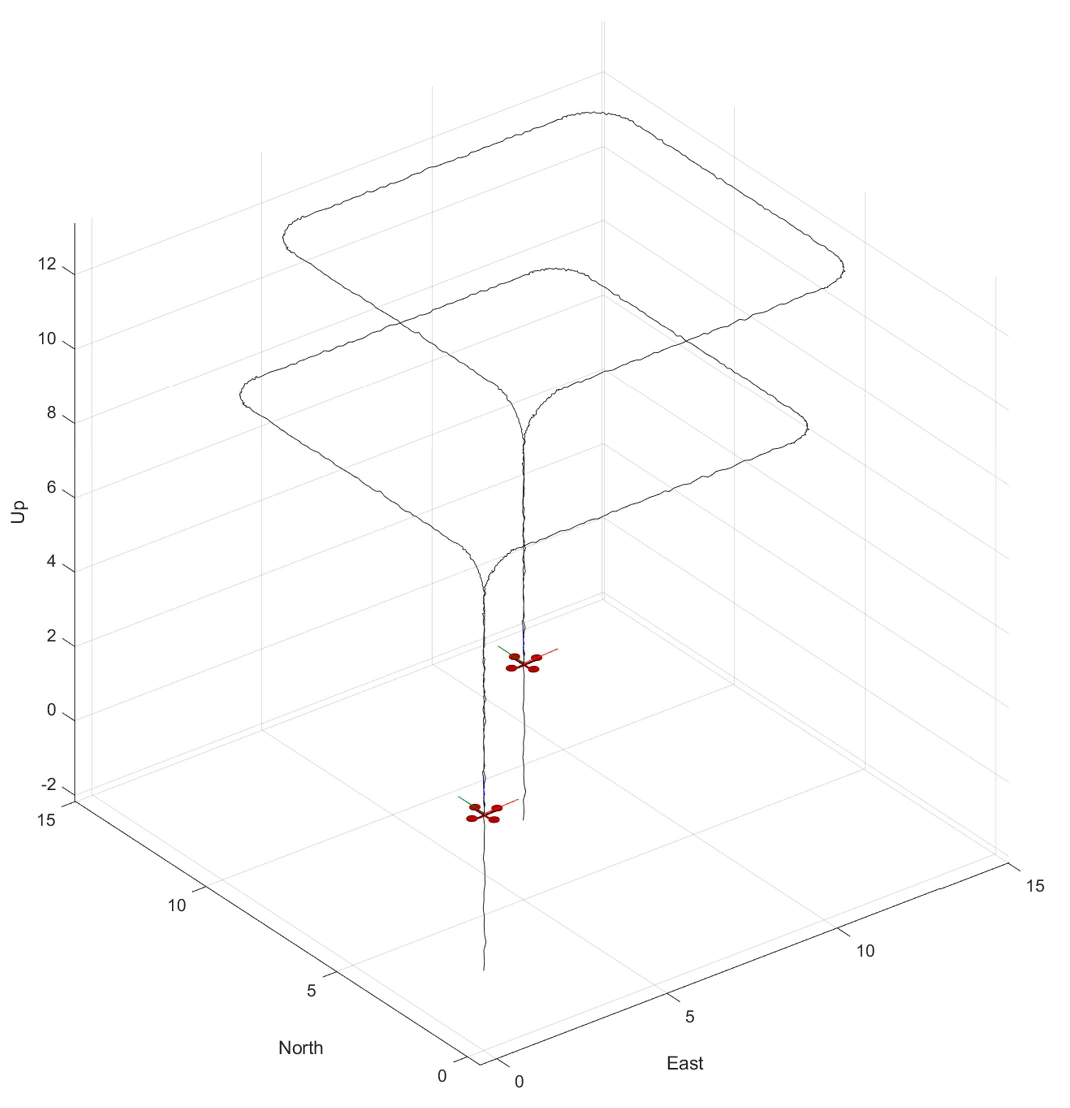
\includegraphics[width=\textwidth]{figs/Samuel/Figures/MultiAgentExampleRed (2).pdf}
        \caption{Multi-agent simulation demonstrating when drones are too close together (distances in metres)}
        \label{fig:1a}
    \end{subfigure}
    \hspace{0.01\textwidth}
    \begin{subfigure}[b]{0.48\textwidth} % Use [b] to align captions at the bottom
        \centering
        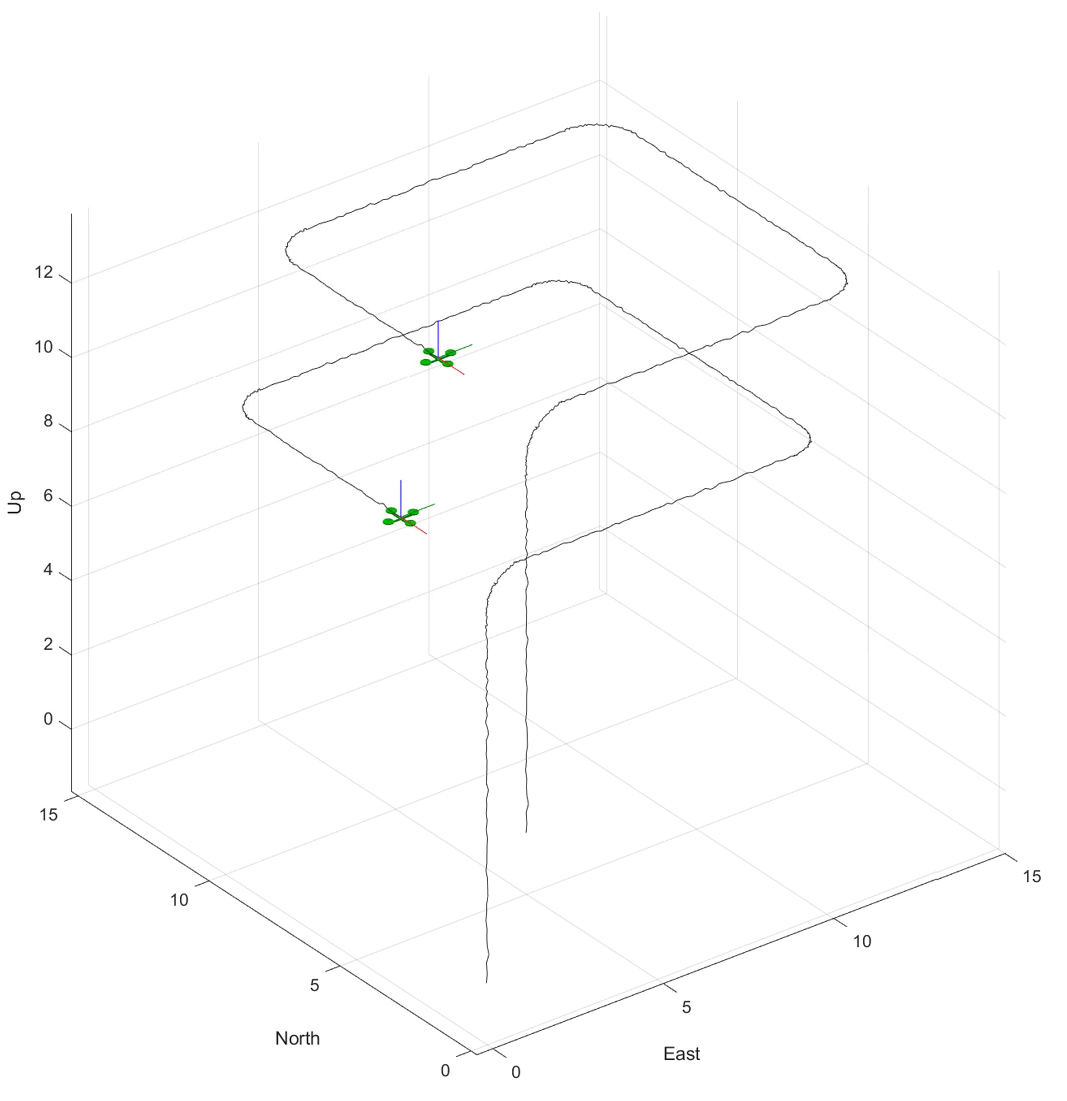
\includegraphics[width=\textwidth]{figs/Samuel/Figures/MultiAgentExampleGreen (2).pdf}
        \caption{Multi-agent simulation demonstrating when drones are a safe distance apart (distances in metres)}
        \label{fig:1b}
    \end{subfigure}
    \caption{Multi-agent simulation with drones too close together (a) and a safe distance apart (b).}
    \label{fig:dronemulti}
\end{figure}

\newpage


\subsection{Wind Gust Prediction using Machine Learning}
\label{gust}
Modelling the effects of wind disturbances is crucial to assessing the viability of a mission. Within the range of acceptable wind speeds, the controller must be sufficiently robust to wind disturbances so that the drone can maintain a steady hovering position. This requirement is necessary because a key constraint on the drone's sensing capabilities is its ability to accurately maintain a set reference condition. The approach taken uses an Application Programming Interface (API) to access current and future weather data for the specified coordinates of the drone's mission, and then takes the maximum wind speed as an input to the simulation. 

The \href{https://www.meteomatics.com/}{\textbf{Meteomatics API}}  is used to find the u, v and w components\footnote{u is positive for a west to east flow, v is positive for a south to north flow and, for w, negative values denote rising motions and positive values denote descending motions} of the wind speed for a given location \cite{meteomatics_wind_speed}. Running these simulations allows a decision to be made in advance as to whether a mission is viable at a particular time. This avoids both unnecessary expense in travelling and setting up for an unfeasible mission and ensures the drone is not damaged due to being operated in hazardous conditions. While the \href{https://www.meteomatics.com/}{\textbf{Meteomatics API}}
provides a valuable forecast of the weather conditions, there is an inherent degree of uncertainty present due to the random nature of gusts of wind. To enhance the drone's robustness against sudden wind gusts, it is crucial to harness artificial intelligence to compute \textbf{online estimates} of incoming gust occurrences. 

\subsubsection{Machine Learning Algorithms}

One of the key constraints on the drone's ability to gather reliable sensor data is how well it can tolerate sudden gusts of wind. Providing the drone with advance warning of when wind gusts are expected would significantly improve the drone's ability to remain stable at all times. The drone is equipped with various sensors, including a gyroscope and an accelerometer. Using the data from these sensors in combination with machine learning algorithms makes it possible to predict when the drone will experience a sudden gust of wind during flight.

To make the gust prediction, a \textbf{binary classifier} is required to decide whether the conditions indicate the presence or absence of an incoming gust. The dataset used to train the machine learning model is labelled, so a \textbf{supervised learning algorithm} is appropriate. The use of drone sensor data in predicting wind gusts has been attempted previously \cite{gu2018wind}. However, this approach will consider the application of additional algorithms which, to the best of the author's knowledge, have not been utilised in this context before. Although deep neural networks (DNN) have now become ubiquitous in the field of machine learning, the dataset being considered here contains too few data samples for DNNs to provide useful results \cite{golestaneh2024samplesneededtraindeep}. Instead, a simpler approach needs to be considered. The rarity of wind gusts means there are fewer data samples with wind gusts present than absent.

The  \textbf{Synthetic Minority Oversampling Technique (SMOTE)} algorithm can be used to improve the performance of a classifier operating on an imbalanced dataset \cite{chawla2002smote}. As is often the case, the real-world dataset for gust conditions contains many datapoints for the absence of a gust, but only a small percentage of the readings correspond to the \textit{interesting case} of the presence of a gust. The use of SMOTE allows for the dataset to be artificially rebalanced, and has the potential to improve the performance of the binary classifier significantly.

In this instance, a basic implementation of the Random Forest Classifier \cite{scikit-learn} is used in Python to classify the data. A labelled dataset is utilised from a previous implementation of drone gust detection \cite{gu2018wind}, and the data is preprocessed by introducing additive Gaussian noise (AGN) to simulate real-world sensor inaccuracies. The data is split using a \textbf{80/20 train-test split}, and the Random Forest model is then trained on the data. To perform a comparative evaluation on the effect of the number of trees used in the random forest, F2 score is used as the performance metric because it prioritises recall (R) over precision (P). The model's F2 score is evaluated while varying the number of trees used. Figure XXX shows the average variation of the F2 score with an increasing number of trees. 

\subsubsection{Evaluation}

Figure \ref{fig:featureimportance} shows the normalised feature importance for each of the measurements used in the machine learning model. The most important feature is the \textbf{gyroscope z axis measurement}. This is expected since it is directly proportional to the angular velocity in the x-y plane, and the drone will rotate about the z-axis when the wind exerts a lateral force. The \textbf{gyroscope x and y axes measurements} are the next most important features, which is to be expected since the wind will also cause the drone to tilt in the x-z and y-z planes. The \textbf{accelerometer measurements} are much less important, as they measure linear motion rather than rotational, and are more sensitive to high frequency noise than gyroscopes \cite{CASSON2016175}. These results suggest that by only using gyroscope measurements an online estimate could be computed more efficiently with minimal accuracy loss.

\begin{figure}[H]
\centering
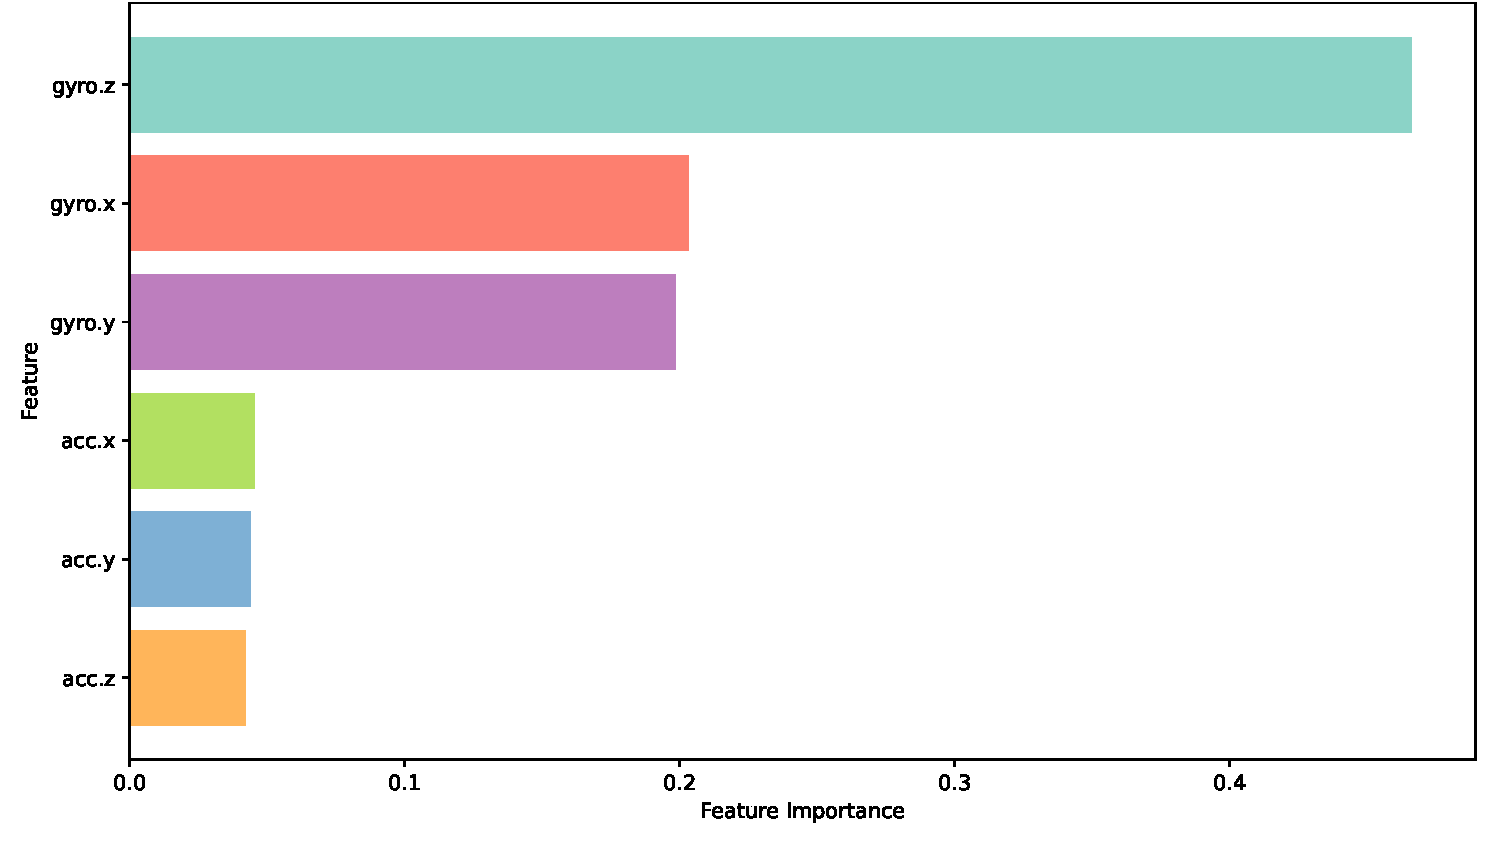
\includegraphics[width=0.8\textwidth]{figs/Samuel/Figures/feature_importance_smote (cropped) (pdfresizer.com).pdf}
\caption{Bar chart showing the normalised feature importance for the Random Forest classifier}
\label{fig:featureimportance}
\end{figure}

The comparison of the model's performance before and after the addition of \textbf{SMOTE} is shown in Figure \ref{fig:smote}. The performance metrics used on the diagram are: proof of concept emphasise why results not gr8

\begin{figure}[H]
\centering
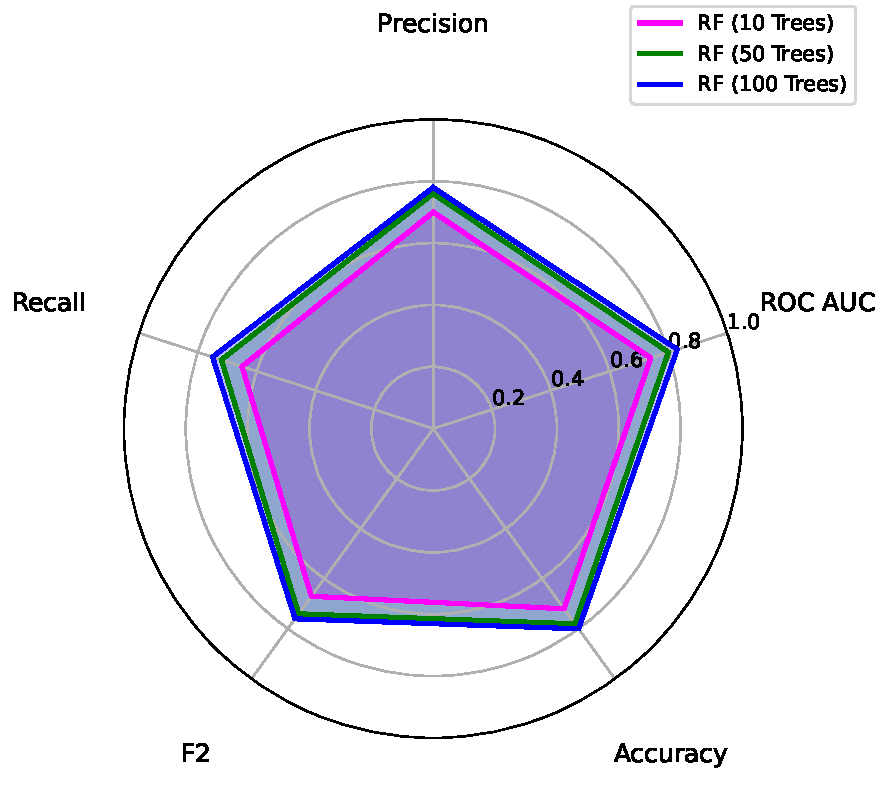
\includegraphics[width=0.7\textwidth]{figs/Samuel/Figures/rf_comparison (1) (cropped) (pdfresizer.com).pdf}
\caption{Radar chart showing the performance of the Random Forest classifier as the number of trees used varies.}
\label{fig:smote}
\end{figure}






\subsection{Embedded Algorithms}

The simulations performed in previous sections help to build confidence as to whether strategies are viable, but the methods chosen must still be implemented onboard the drone. There are numerous options for implementing processes on a drone, with the most common and well-documented being the use of embedded C code on a microcontroller. For these reasons, all of the processes carried out onboard the drone use a microcontroller running embedded C code. The algorithms are tested using the ARM GNU Toolchain, 

\subsubsection{\gls{bms} Algorithms}

The algorithms required to implement the \gls{bms} are run onboard an \textbf{STM32F405} microcontroller, with the MATLAB Coder used to convert all of the required processes into embedded C code. The Coder is configured to optimise the converted algorithms for the \textbf{STM32F405}, since it is specified as the \textit{target hardware}. The exceptions to this method are the Kalman filtering algorithms, which utilise a pre-optimised C library, as discussed in Section \ref{kalm}.

\subsubsection{Cascade \gls{pid} Control}

The cascade \gls{pid} control system designed is implemented onboard the drone using a controller which has been specifically designed in C for the STM32H7 board. https://github.com/ChrisWonyeobPark/PID-Control/blob/master/PID\%20control.c


\subsubsection{ML}

The Random Forest model is implemented using a lightweight C library to allow for efficient operation. 

https://github.com/andriidski/random-forests-c/tree/master

\newpage

\subsection{Future Work}

\subsubsection{Control Techniques}

Despite cascade \gls{pid} being simpler to implement and easier to modify than most other control strategies, the ongoing increase in microcontroller processing power will enable more sophisticated methods to be implemented onboard the drone. The first potential improvement could be made by combining the \gls{lqr} and \gls{pid} control techniques onboard the drone, so that the drone can benefit from the robustness of the \gls{pid} controller in general flight, while being able to hover more steadily using a finely tuned \gls{lqr}. \gls{mpc} could also be investigated to allow the drone's controller to be updated during the mission, although this method would require a significant increase in onboard processing power. Backstepping could also be investigated, which involves dividing the system into smaller subsystems and designing the overall control scheme recursively, allowing the full nonlinear system to be modelled while ensuring that Lyapunov stability is satisfied \cite{4058900}. Designing model-free controllers by leveraging the power of machine learning techniques is also an ongoing area of research, which would also allow for the system's dynamics to be more accurately modelled. All of these techniques have the potential to improve the flight controller's performance, but introduce additional complexity and cost to the theoretical model and the embedded code.

\subsubsection{ML}

The machine learning model discussed in this report serves as a proof of concept for online gust detection; the limited size of the dataset available acted as a constraint on the models that could be employed. Deploying the model onboard a drone to evaluate its effectiveness and gathering a larger labelled dataset would be required to further develop this idea. Significant improvements would likely be achievable if a sufficiently large dataset was used to train a \gls{dnn}. Alternatively, the problem could be recast as a \textbf{regression} problem, where the model predicts the speed of the incoming gust rather than simply its occurrence. Solving this problem would again require a significantly large dataset, but would provide more informative predictions. 

\newpage

